\documentclass[a4paper, 12pt]{book}

\usepackage[T1]{fontenc}
\usepackage[utf8]{inputenc}
\usepackage[italian]{babel}
\usepackage{quoting}
\usepackage{graphicx} %per inserire immagini nel testo
\usepackage{sidecap} %permette di aggiungere didascalie alle immagini
\usepackage{subfig}
\usepackage[colorlinks]{hyperref} %per rendere interattivo il documento, gli elementi interattivi saranno in rosso con l'opzione colorlinks
\usepackage{amsmath}
\usepackage{amsthm} %per enunciati
\theoremstyle{plain}
\newtheorem{teorema}{Teorema}[section]
\usepackage{geometry}
\geometry{a4paper, top = 3cm, bottom = 3cm, left = 3.5cm, right = 3.5cm, heightrounded, bindingoffset = 5mm}
\pagestyle{plain}
\usepackage{multirow}
\setcounter{secnumdepth}{3}

\title{Sistemi}
\author{Giovanni Tosini}
\date{ }

\begin{document}

\begin{titlepage}
    \maketitle
\end{titlepage}

\frontmatter
\tableofcontents
\mainmatter

\chapter{Numeri complessi}

Un numero complesso $s = \sigma + j\omega$ con $j = \sqrt{-1}$ e $\sigma , \omega \in R$ in cui 
\begin{itemize}
    \item $\sigma = Re(s)$ parte reale
    \item $\omega = Im(s)$ parte immaginaria
    \item $C = {s t.c. s = \sigma + j\omega, \sigma , \omega \in R}$ insieme dei numeri complessi
\end{itemize}
\begin{center}
    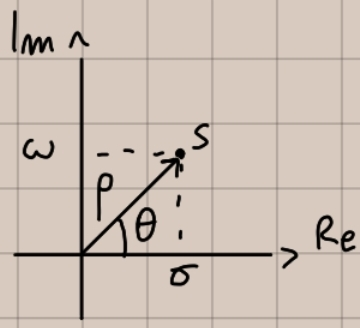
\includegraphics[width=0.5\textwidth]{num_comp.jpg}
\end{center}
Forma polare dei numeri complessi, $s = \rho (cos\theta +jsin\theta)$
\begin{itemize}
    \item $\rho = \sqrt{\sigma ^2+\omega ^2}$ il modulo di $s$ con $\rho \in R^+$
    \item $\theta =$ argomento di $s$
\end{itemize}
\begin{description}
    \item[Osservazione 1] $Re(s) = \rho cos\theta$ e $Im(s) = \rho sin\theta$
    \item[Osservazione 2] L'argomento $\theta$ è determinato a meno di multipli interi di 
            $2\pi$. Imponendo $\theta \in [0, 2\pi )$ oppure $(-\pi , \pi ]$ (deve essere un intervallo
            lungo $2\pi$ ) si ottiene l'argomento principale $\theta$ che notiamo con $arg(s)$  
\end{description}

\section{Formula di Eulero}

$\theta \in R, j = \sqrt{-1}$ abbiamo $e^{j\theta}=cos\theta +jsin\theta$

\paragraph{Forma esponenziale}

$s=\rho e^{j\theta}$
\begin{center}
    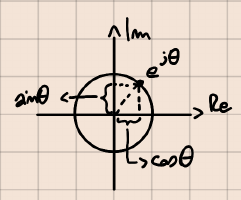
\includegraphics[width=0.5\textwidth]{num_comp2.png}
\end{center}
$|e^{j\theta}=\sqrt{cos^2\theta +sin^2\theta} = 1$

Esempio: $e^{j\frac{\pi}{2}}=j$
\begin{center}
    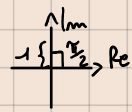
\includegraphics[width=0.5\textwidth]{num_comp3.png}
\end{center}
$s=0+1j=j$
\begin{description}
    \item[Def:] i numeri \textbf{immaginari puri} hanno la parte reale nulla
    \item[Def:] dato $s: \sigma + j\omega \in C$ $\bar{s}: \sigma - j\omega$ coniugato complesso   
\end{description}
\begin{center}
    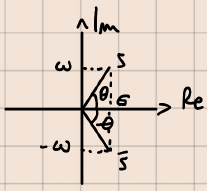
\includegraphics[width=0.5\textwidth]{num_comp4.png}
\end{center}
La forma polare di $\bar{s}$ sarà uguale a $\rho (cos\theta - jsin\theta)$
\begin{description}
    \item[Osservazione] $|s|=|\bar{s}| arg(\bar{s})=-arg(s)$ 
\end{description}

Esempio: $e^{j\pi}=-1=e^{j\pi}+1=0$
\begin{center}
    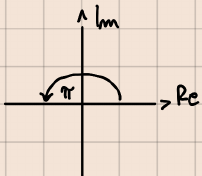
\includegraphics[width=0.5\textwidth]{num_comp5.png}
\end{center}

\section{Operazioni con i numero complessi}

\begin{itemize}
    \item $s_1=\sigma_1+j\omega_1,s_2=\sigma_2+j\omega_2\in C$
    \item $s_1+s_2=\sigma_1+\sigma_2+j(\omega_1+\omega_2)$
    \item $s_1-s_2=\sigma_1-\sigma_2+j(\omega_1-\omega_2)$
\end{itemize}
\begin{description}
    \item[Osservazione:] $Re(s)=\frac{s+\bar{s}}{2}$ e $Im(s)=\frac{s+\bar{s}}{2j}$ 
\end{description}
Per la formula di Eulero $e^{j\theta}=cos\theta+jsin\theta \Rightarrow cos\theta = \frac{e^{j\theta}+e^{-j\theta}}{2}$ e
$sin\theta =\frac{e^{j\theta} -e^{-j\theta}}{2j}$
\begin{center}
    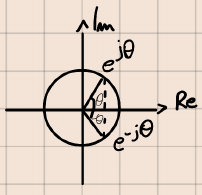
\includegraphics[width=0.5\textwidth]{num_comp6.png}
\end{center}
\begin{description}
    \item[Osservazione:]$2Re(s)=s+\bar{s}$ e $2jIm(s)=s-\bar{s}$ 
\end{description}
$s=\bar{s} \Rightarrow Im(s)=0$ e $s=-\bar{s} \Rightarrow Re(s)=0$
\begin{center}
    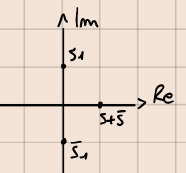
\includegraphics[width=0.5\textwidth]{num_comp7.png}
    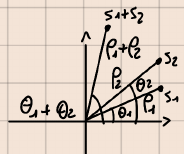
\includegraphics[width=0.5\textwidth]{num_comp8.png}
\end{center}
\begin{itemize}
    \item $s_1 = \rho_1(cos\theta_1+jsin\theta_1)$
    \item $s_2 = \rho_1(cos\theta_2+jsin\theta_2)$
    \item $s_1s_2=\rho_1\rho_2(cos(\theta_1+\theta_2)+jsin(\theta_1+\theta_2))$
    \item $s_1s_2=\rho_1\rho_2(cos\theta_1cos\theta_2+jcos\theta_1sin\theta_2+jsin\theta_1cos\theta_2-sin\theta_1sin\theta_2)$
    \item $s_1s_2=\rho_1\rho_2(cos\theta_1cos\theta_2-sin\theta_1sin\theta_2+j(cos\theta_1sin\theta_2+sin\theta_1cos\theta_2))$
\end{itemize}
\begin{description}
    \item[N.B.:] $cos\theta_1cos\theta_2-sin\theta_1sin\theta_2=cos(\theta_1+\theta_2)$ e 
    $cos\theta_1sin\theta_2+sin\theta_1cos\theta_2=sin(\theta_1+\theta_2)$
    \item [Def:]Dato $s\in C$ il numero $s^{-1}$ t.c. $ss^{-1}=1$, $s^{-1}=\frac{\bar{s}}{|s|^2}$ reciproco
    (inverso) di $s$.
    \item $ss^{-1}=s\frac{\bar{s}}{|s|^2}=\frac{s\bar{s}}{|s|^2}$
    \item $s\bar{s}=\rho^2(cos(\theta-\theta)+jsin(\theta-\theta))=\rho^2=|s|^2$
    \item [Osservazione:]l'argomento di un numero complesso si può chiamare anche \textbf{fase}.
    \item $\frac{s_1}{s_2}=s_1s_2^{-1}=s_1\frac{\bar{s_2}}{|s_2|^2}=\frac{\rho_1}{\rho_2}(cos(\theta_1-\theta_2)
    jsin(\theta_1-\theta_2))$
    \item [Osservazione:] $s\bar{s}=\rho^2(cos(\theta-\theta)+jsin(\theta-\theta))=\rho^2\Rightarrow|s|^2=s\bar{s}$ 
\end{description}
\begin{center}
    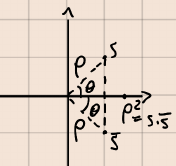
\includegraphics[width=0.5\textwidth]{num_comp9.png}
\end{center}
\begin{description}
    \item[Def: ]$u\in C$ si dice complesso unitario se $|u|=1$. In forma polare $u=cos\theta+jsin\theta$. In forma esponenziale
     $u=e^{j\theta}$ e $|e^{j\theta}|=1$  
\end{description}
Sia $u=cos\alpha+jsin\alpha$ con $s=\rho(cos\theta+jsin\theta)$ avremo che $su=\rho(cos(\theta+\alpha)+jsin(\theta+\alpha))$
(rotazione intorno all'origine)
\begin{center}
    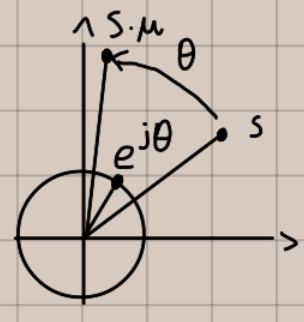
\includegraphics[width=0.5\textwidth]{num_comp10.jpg}
\end{center}
$s^n=\rho^n(cos(n\theta)+jsin(n\theta))$

Esempio: \[(e^{j\theta})^n=e^{jn\theta}\]
\paragraph{Radici complesse}

Ogni $s\in C$ ammette $n$ distinte radici $n$-esime $\omega_1,\dots,\omega_{n-1} \in C$.
Dobbiamo trovare $\omega \in C$ t.c. $\omega^n=s$.
\[]\forall k \in [0, n-1], \omega_k\sqrt[n]{\rho}(cos(\frac{\theta}{n}+\frac{2\pi}{n}k)
+jsin(\frac{\theta}{n}+\frac{2\pi}{n}k))
\]
Prova: 
\[
\begin{split}
\omega_k^n &= (\sqrt[n]{\rho}^n)(\cos(n(\frac{\theta}{n}+\frac{2\pi}{n}k))+jsin(n(\frac{\theta}{n}+\frac{2\pi}{n}k))) = \\
 &= \rho(cos(\theta+2\pi k)+jsin(\theta+2\pi k))= \\
\end{split}
\]
Notare che $cos(\theta+2\pi k)$ è equivalente a $cos\theta$ e $sin(\theta+2\pi k)$ equivale a $sin\theta$ questo
$\forall k=0,...,n-1$.

L'equazione: $s^4=1+2j$ ha 4 radici distinte nel campo $C$.
Esempio: le radici complesse dell'unità

$s^n=1 \omega_k=cos(\frac{2\pi}{n}k) + jsin(\frac{2\pi}{n}k) k=0,...,n-1$

\paragraph{Funzioni di variabile complessa}

Gli insieme su cui definiamo una funzione di variabile complessa
 f si scrivono $D(f)$, $D(f)\subseteq C$
 \begin{description}
     \item[Def: ]un punto $s_0\in D(f)\subseteq C$ è interno a $D(f)$
     se esiste un disco $B_\rho(s_0)$ di raggio $\rho$ con $\rho\in R^+$ centrato
     in $s_0$, t.c. $B_\rho(s_0)\subseteq D(f)$ dove $B_\rho(s_0)={s\in C t.c. |s-s_0| < \rho}$
 \end{description}
 \begin{center}
     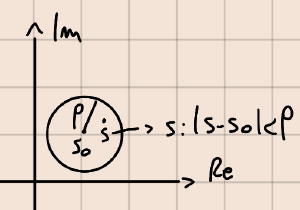
\includegraphics[width=0.5\textwidth]{num_comp11.png}
 \end{center}
 \begin{description}
     \item[Def: ]Un insieme $D(f)\subseteq C$ si dice aperto se tutti i suoi punti
     sono interni 
     \item [Def: ]Una funzione $f:D(f)\rightarrow C$ con $D(f)\subseteq C$ aperto
     è una funzione complessa
 \end{description}
 Esempi di funzioni complesse con annesso dominio:
 \begin{itemize}
     \item $f(s) = s, D(f) = C$
     \item $f(s)=s^2,D(f)=C$
     \item $f(s)=Re(s)+jIm(s)^2, D(f)=C$
     \item $f(s)=\sum_{k=0}^n a_ks^k, D(f)=C$
     \item funzione polinomiale, $f(s)=\frac{P(s)}{Q(s)}$ dove $P(s)=\sum_{k=0}^n a_ks^k$ e funzione razionale $Q(s)=\sum_{k=0}^n b_ks^k$,
     $D=C-{\lambda_1,...,\lambda_m}$ dove $\lambda_\alpha$ è radice di $Q(s)=0$ per $k=1,...,m$
 \end{itemize}
 \section{Teorema fondamentale dell'algebra}
 Ogni polinomio $P(s)$ a coefficienti complessi di grado $n>0$ ha $n$ radici complesse e si può comporre come
 \begin{center}
         $P(s) = a_n(s-\lambda_1)^\mu_1(s-\lambda_2)^\mu_2...(s-\lambda_r)^\mu_r$ dove 
        $\lambda_1,...\lambda_r$ sono radici  e $\mu_1,...,\mu_r$ sono le \textbf{molteplicità} relative di ciascuna
        radice per cui $\mu_1 + ... + \mu_r = n$
 \end{center}
 \begin{description}
     \item[Osservazione] Un numero $\lambda$ è una radice di molteplicità $\mu$ per un polinomio $P(s)$
    se e solo se $P(\lambda)=P'(\lambda)=P''(\lambda)=...=P^{\mu - 1}(\lambda) = 0$ e $P^\mu (\lambda)\neq 0$
    \end{description}

\chapter{Segnali}

Sono funzioni matematiche definite su un dominio, esistono nel dominio:
\begin{itemize}
    \item continuo $\rightarrow R, C, \dots$;
    \item discreto $\rightarrow Z$.
\end{itemize}

\section{Segnali elementari a tempo continuo}
\subsection{Segnale sinusoidale}
Consiste di una funzione:
\[
v: R \rightarrow R, v(t) = A \overbrace{\cos}^{[-1, 1]}(\omega t + \phi)
\textrm{ con } A, \omega, \phi \in R 
\]
\begin{itemize}
    \item $A > 0$ è l'ampiezza;
    \item $\omega$ la pulsazione;
    \item $\phi$ la fase;
    \item $v$ è periodico di periodo $T = \frac{2\pi}{\omega}$;
    \item la frequenza $f = \frac{1}{T} \rightarrow f = \frac{\omega}{2\pi}$.
\end{itemize}

\begin{SCfigure}[50][h!]
    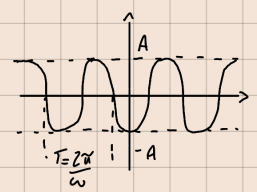
\includegraphics[width=0.5\textwidth]{sinusoidale.png}
    \caption{Funzione sinusoidale}
\end{SCfigure}

\subsection{Fasore}
Una funzione:
\[
v : R \rightarrow C, v(t) = A e^{j(\omega t + \phi)}\footnote{$e^{j\theta} = \cos \theta + j\sin \theta \rightarrow
|e^{j\theta}| = 1$} 
\textrm{ con } A, \omega, \phi \in R    
\]
Di conseguenza sarà uguale sempre ad $A$.
\begin{description}
    \item[Osservazione: ] dalla formulla di Eulero, possiamo esprimere
    un segnale sinusoidale \[\begin{split}
        A \cos (\omega t + \phi) &= A\frac{e^{j(\omega t + \phi)} + e^{-j(\omega t + \phi)}}{2} = \\
        &= \frac{A}{2} e^{j(\omega t + \phi)} + \frac{A}{2} e^{-j(\omega t + \phi)} \\
    \end{split} \]  
\end{description}

\begin{SCfigure}[50][h!]
    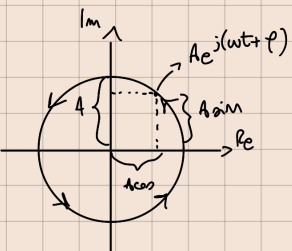
\includegraphics[width=0.5\textwidth]{fasore.png}
    \caption{Fasore}
\end{SCfigure}

\subsection{Segnale sinusoidale modulato esponenzialmente}

\begin{gather}
    v : R \rightarrow R\\
    v(t) = A e^{\sigma t} \cos (\omega t + \phi)\\
    \textrm{ con } \sigma, A, \omega, \phi \in R, A > 0\\
\end{gather}
 \textbf{non} è periodico.   

\begin{itemize}
    \item per $\sigma > 0$ e $t \rightarrow \infty \Rightarrow v(t) = \infty$
    \item per $\sigma < 0$ e $t \rightarrow \infty \Rightarrow v(t) = 0$
\end{itemize}

\begin{SCfigure}[50][h!]
    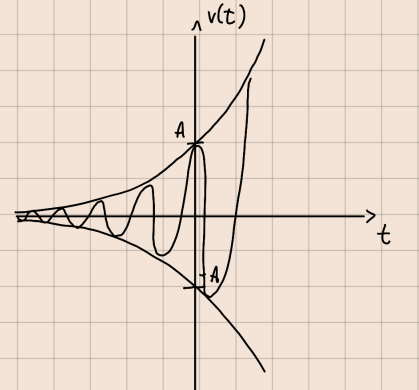
\includegraphics[width=0.3\textwidth]{nomelunghissimo.png}
    \caption{Segnale sinusoidale modulato esponenzialmente}
\end{SCfigure}

\begin{description}
    \item[Osservazione: ] segnali sinusoidali, modulati esponenzialmente, si possono scrivere come combinazione lineare di fasori con una componente esponenziale: \[
        \begin{split}
            A e^{\sigma t} \cos (\omega t + \phi) &= A e^{\sigma t} \frac{e^{j(\omega t + \phi)} + e^{-j(\omega t + \phi)}}{2} = \\
            &= \frac{A e^{\sigma t} e^{j(\omega t + \phi)}}{2} + \frac{A e^{\sigma t} e^{-j(\omega t - \phi)}}{2} = \\
            &= \underbrace{\frac{A}{2} e^{\sigma t} e^{j\omega t + j\phi} + \frac{A}{2} e^{\sigma t} e^{-j\omega t - j\phi}}_{\textrm{sono complessi coniugati}}
        \end{split}
         \] 
\end{description}

\subsection{Segnale esponenziale complesso}
\[
v : R \rightarrow C, v(t) = A e^{\sigma t} e^{j(\omega t + \phi)}
\]

\begin{figure}[h!]
    \centering
		\subfloat[][\textbf{\emph{Per $\sigma > 0$ e $t \rightarrow \infty |v(t)| \rightarrow \infty$}}]
		{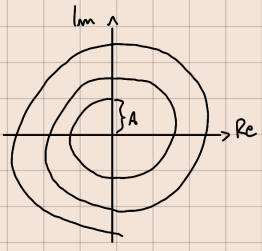
\includegraphics[width=0.3\textwidth]{uzumaki1.png}}\quad
		\subfloat[][\textbf{\emph{Per $\sigma < 0$ e $t \rightarrow \infty |v(t)| \rightarrow 0$}}]
		{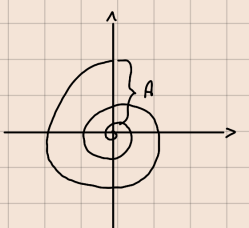
\includegraphics[width=0.3\textwidth]{uzumaki2.png}}\\
\end{figure}

\subsection{Funzioni generalizzate}
\subsubsection{Segnali polinomiali}
\[
\delta_{-n} : R \rightarrow R \\
\delta_{-n} = \begin{cases}
    \frac{t^{n - 1}}{(n - 1)!}, t \ge 0;\\
    0 \textrm{, altrimenti}
\end{cases}    
\]

Da un certo istante ha un valore e quello sarà l'istante 0.
\begin{description}
    \item[Osservazione: ] \[
    \delta_{-n}(t) = \int_{-\infty}^t \delta_{-(n - 1)}(\Psi)d\Psi    
    \] 
    Il segnale polinomiale n-esimo può essere ottenuto come integrale del segnale (n - 1)-esimo
    \[
    \delta_{-n}(t) = \frac{d\delta_{-(n + 1)}^t}{dt}\]
\end{description}
Esempio per n = $1$
\[\delta_{-1}(t) = 
\begin{cases}
    1, t \ge 0\\
    0, \textrm{altrimenti}
\end{cases}    
\]

Per n = $2$
\[\delta_{-2}(t) =
\begin{cases}
    t, t \ge 0\\
    0, \textrm{altrimenti}
\end{cases}
\]

\begin{figure}[h!]
    \centering
		\subfloat[][\textbf{\emph{Funzione gradino}}]
		{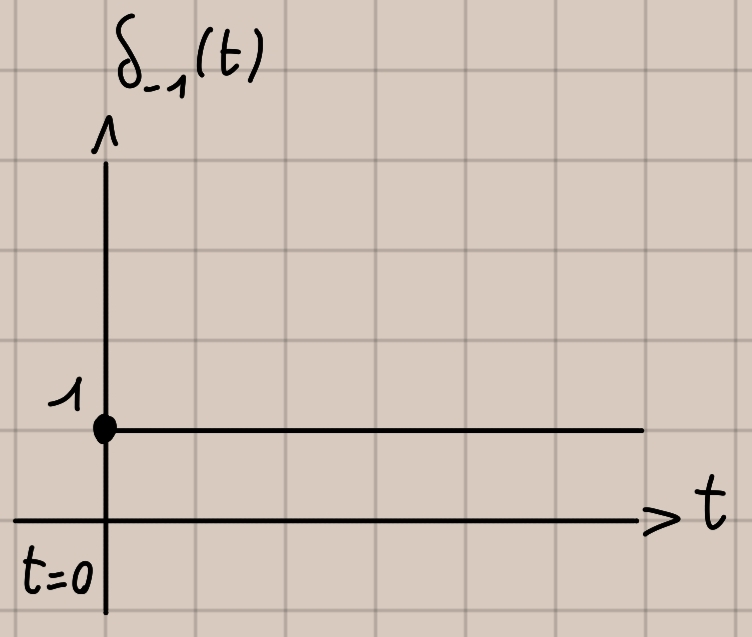
\includegraphics[width=0.3\textwidth]{gradino.jpg}}\quad
		\subfloat[][\textbf{\emph{Rampa unitaria}}]
		{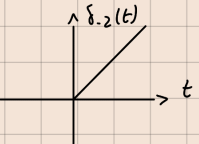
\includegraphics[width=0.3\textwidth]{rampa.png}}\\
\end{figure}

\begin{description}
    \item[Osservazione: ] l'integrale del gradino è la rampa e viceversa la derivata della rampa è il gradino.
\end{description}
\[
    \int_{-\infty}^{t}\delta_{-1}d\alpha = \delta_{-2}(t) \\
    \frac{d\delta_{-2}(t)}{dt} = \delta_{-1}(t)  
\]

\subsubsection{Finestra rettangolare unitaria}

\[
    \Pi : R \rightarrow R \Pi(t) = \begin{cases}
        1, -\frac{1}{2} \le t \le \frac{1}{2}\footnote{Il supporto = $(-\frac{1}{2}, \frac{1}{2}) \subset R$}\\
        0, \textrm{altrimenti}
    \end{cases}    
\]

\begin{SCfigure}[50][h!]
    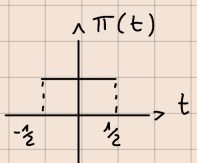
\includegraphics[width=0.3\textwidth]{finestra.png}
    \caption{Finestra rettangolare unitaria, ampiezza = $1$}
\end{SCfigure}

\begin{description}
    \item[Osservazione: ] La finestra rettangolare unitaria è una combinazione lineare di due gradini: 
\end{description}

\[
    \Pi(t) = \delta_{-1}(t + \frac{1}{2}) - \delta_{-1}(t - \frac{1}{2})
\]

\subsubsection{Finestra rettangolare ad ampiezza A con diverso supporto}

\begin{description}
    \item[N.B.:] il supporto è il sottoinsieme del dominio per cui la funzione è $\neq 0$
\end{description}

\begin{center}
    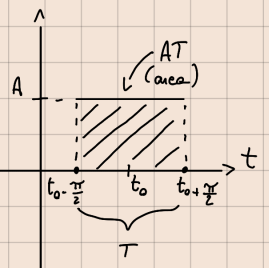
\includegraphics[width=0.3\textwidth]{finestra2.png}
\end{center}

L'ampiezza A, centrata in $t_0$, con supporto $(t_0 - \frac{\pi}{2}, t_0 + \frac{\pi}{2})$.
\[
    A\Pi(\frac{t - t_0}{T}) = \begin{cases}
        A, t_0 - \frac{\pi}{2} \le t \le t_0 + \frac{\pi}{2}\\
        0, \textrm{altrimenti}
    \end{cases}
\]

\subsubsection{Finestre (o impulso) triangolare unitaria}

\[
    \Lambda : R \rightarrow R, \Lambda(t) = \begin{cases}
        1 - |t|, -1 \le t \le 1\\
        0, \textrm{altrimenti}
    \end{cases}
\]

\begin{SCfigure}[50][h!]
    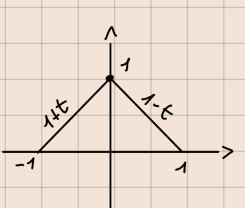
\includegraphics[width=0.3\textwidth]{triangolo.png}
    \caption{Impulso, supporto $[-1, 1]$, area = $1$}
\end{SCfigure}

\subsubsection{Finestra triangolare ad ampiezza A con supporto 2T centrata in $t_0$}

\begin{center}
    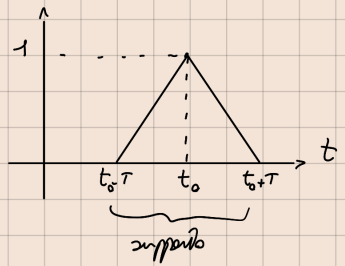
\includegraphics[width=0.5\textwidth]{triangolo2.png}
\end{center}

\[
    A\Lambda(\frac{t - t_0}{T}) = \begin{cases}
        A - \frac{A}{T} |t - t_0|, t_0 - T \le t \le t_0 + T\\
        0, \textrm{altrimenti}
    \end{cases}
\]
supporto $(t_0 - T, t_0 + T)$, area = $AT$

\subsubsection{Impulso di Dirac o funzione $\delta (t)$}
\begin{description}
    \item[Osservazione: ] l'impulso è una funzione generalizzata che è definita come un limite di una succesione di funzioni. 
\end{description}

\[
    \begin{split}
        \delta(t) &= \lim_{n \rightarrow \infty} \delta_n (t) =\\
        &= \lim_{n \rightarrow \infty} \frac{n}{2}\Pi(\frac{t}{\frac{2}{n}}) \textrm{ dove}\\
        f_n(t) &= \frac{n}{2}\Pi(\frac{t}{\frac{2}{n}}) = \\
        &=\begin{cases}
            \frac{n}{2}, -\frac{1}{n} \le t \le \frac{1}{n}\\
            0, \textrm{altrimenti}
        \end{cases}
    \end{split}  
\]

\begin{SCfigure}[50][h!]
    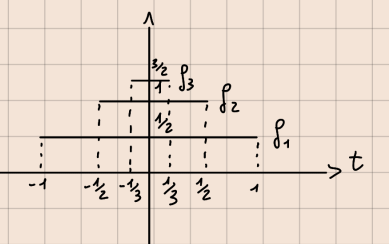
\includegraphics[width=0.5\textwidth]{dirac.png}
    \caption{Impulso di Dirac, prosegue fino a $\infty$}
\end{SCfigure}

\[
    \delta_t "=" \begin{cases}
        \infty, t = 0\\
        0, \textrm{altrimenti}
    \end{cases}
\]
\[
    \begin{split}
        \int_{-\infty}^\infty \delta(t) dt &= \int_{-\infty}^\infty \lim_{n \rightarrow \infty} f_n(t) dt = \\
        &= \lim_{n \rightarrow \infty} \int_{-\infty}^\infty \overbrace{f_n (t) dt}^{\textrm{ogni finestra ha area = 1}} = \\
        &= \lim_{n \rightarrow \infty} 1 = 1
    \end{split}
\]

\begin{SCfigure}[50][h!]
    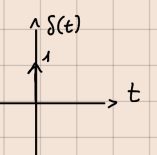
\includegraphics[width=0.5\textwidth]{frecciasu.png}
    \caption{Rappresentazione grafica}
\end{SCfigure}

\subsubsection{Impulso di ampiezza A e centrato in $t_0$}

\[
    A\delta(t - t_0) = \begin{cases}
        \infty, t = t_0\\
        0, \textrm{altrimenti}
    \end{cases}    
    \int_{-\infty}^{\infty0} A\delta(t - t_0) dt = A
\]
Proprietà dell'impulso:
\begin{itemize}
    \item L'impulso ideale centrato in origine è pari a: \[\delta(-t) = \delta(t), t \in R\]
    \item Area unitaria \[\begin{cases}
        \int_a^b \delta(t)dt = 1, \textrm{ se } 0 \in (a, b)\\
        \int_a^b \delta(t)dt = 0, \textrm{ altrimenti}\\
    \end{cases}\]
    \item Proprietà di campionamento
\end{itemize}

\begin{center}
    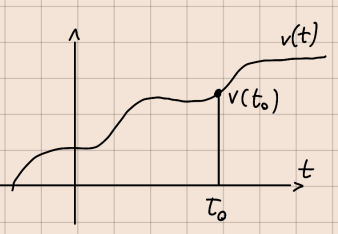
\includegraphics[width=0.5\textwidth]{campionamento.png}
\end{center}

\[
    v(t_0) = \int_{-\infty}^\infty v(t) \delta(t - t_0) dt    
\]

Inolte se v è continua sul dominio 
\[
    V(t) =   \int_{-\infty}^\infty v(t) \delta(t - t) dt \textrm{ moltiplico per } \delta(t - t_0)
\]
\textbf{Dimostrazione}:  
\[
    \begin{split}
        v(t_0) &= v(t) + v(t_0) - v(t)\\
        &v(t_0) \delta(t- t_0) = v(t) \delta(t - t_0) + [v(t_0) - v(t)] \delta(t - t_0)\\
        &\int_{-\infty}^\infty v(t_0) \delta(t - t_0)dt =\\
        &\int_{-\infty}^\infty v(t) \delta(t - t_0) dt +\\
        &+ \underbrace{\int_{-\infty}^\infty \overbrace{\delta(t - t_0)}^{0 \textrm{ per } t \neq t_0} \overbrace{[v(t_0) - v(t)]}^{0 \textrm{ per } t = t_0}}_0dt\\
        &\Rightarrow v(t_0) \underbrace{\int_{-\infty}^\infty \delta(t - t_0) dt}_{1 \textrm{ perché l'impulso è unitario}} = \\
        &= \int_{-\infty}^\infty v(t) \delta(t - t_0) dt\\
        v(t_0) &= \int_{-\infty}^\infty v(t) \delta(t - t_0) dt
    \end{split}    
\] 
\begin{description}
    \item[Osservazione: ] si può scrivere anche come \[v(t_0)  = v(t) \delta (t - t_0)\] 
\end{description}

\section{Segnali a tempo discreto}

\subsection{Impulso unitario discreto o delta di Kroneker}

$\delta: Z \rightarrow R$ è una successione
\[\delta(k) = 
    \begin{cases}
        1, \textrm{ per } k = 0\\
        0, \textrm{ altrimenti}
    \end{cases}  
\]

\begin{SCfigure}[50][h!]
    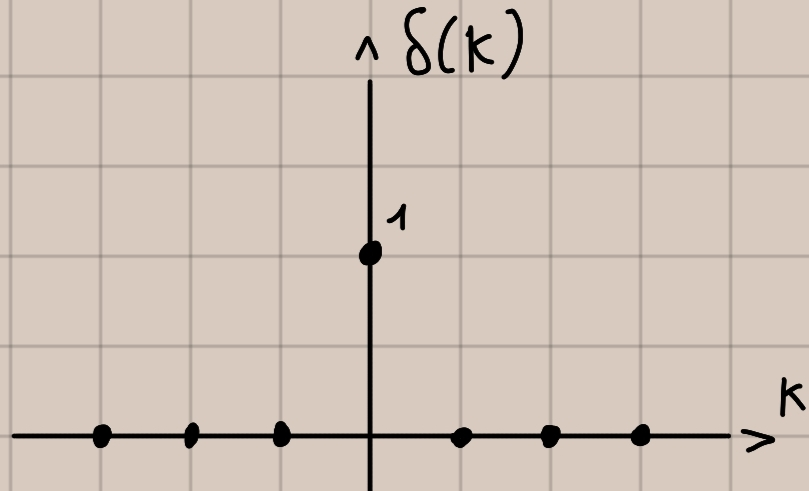
\includegraphics[width=0.5\textwidth]{kroneker.jpg}
    \caption{Delta di Kroneker}
\end{SCfigure}

\subsection{Gradino unitario discreto}

\[
    \delta_{-1}: Z \rightarrow R\qquad \delta_{-1} = \begin{cases}
        1, k \ge 0\\
        0, \textrm{ altrimenti}
    \end{cases}
\]

\begin{SCfigure}[50][h!]
    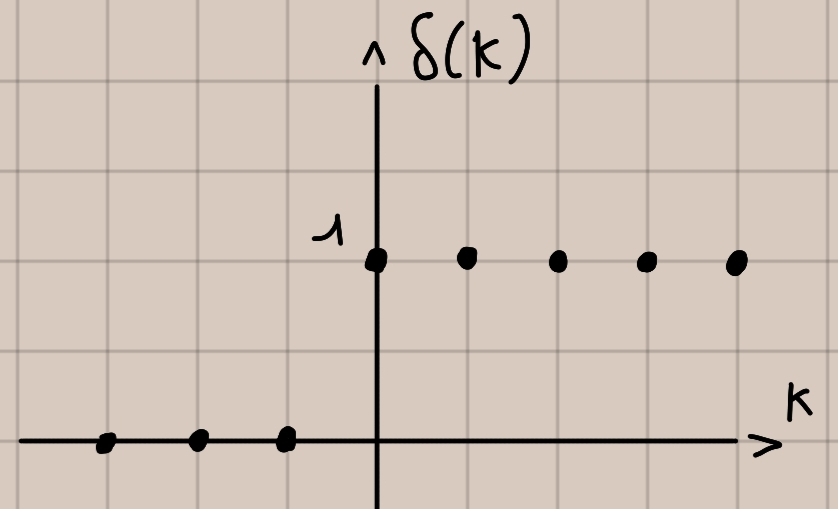
\includegraphics[width=0.5\textwidth]{gradino2.jpg}
    \caption{Gradino}
\end{SCfigure}

\subsection{Rampa discreta unitaria}

\[
    \delta_{-2}: Z \rightarrow R:\qquad \delta_{-2} = \begin{cases}
        k, k \ge 0\\
        0, \textrm{ altrimenti}
    \end{cases}
\]

\begin{SCfigure}[50][h!]
    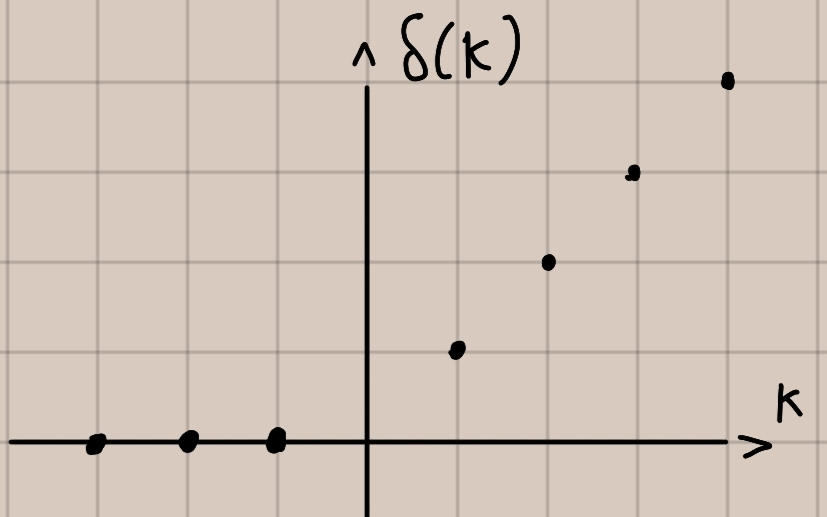
\includegraphics[width=0.5\textwidth]{rampa2.jpg}
    \caption{Rampa}
\end{SCfigure}

\begin{description}
    \item[Osservazione: ] abbiamo che l'integrale dell'impulso del gradino, come serie corrisponde a $\delta_{-1}(k) = \sum_{i = -\infty}^k \delta(i)$ praticamente se io sommo tutti 
    tutti i valori dell'impulso avrò come risultato un qualsiasi valore $k \ge 0$, sommando tutti i valori dell'impulso ottengo il gradino e in modo analogo sommando tutti i valori 
    del gradino fino a k ottendo la rampa $\delta_{-2} = \sum_{i = -\infty}^{k - 1} \delta_{-1} (i)$.
    \item[N.B.: ] la somma nel campo discreto corrisponde all'integrazione nel campo continuo. 
\end{description}

\[
    \delta_{-2} (k) = \sum_{i = -\infty}^{k - 1} \sum_{j = -\infty}^i \delta(ij)
\]

\subsection{Successione esponenziale discreta}

\[
    v : Z \rightarrow R,\quad v(k) = A e^{j\phi} \lambda^k, \textrm{ dove } k \in Z, \phi \in R,\lambda \in C.   
\]
\begin{description}
    \item[Osservazione: ] se scriviamo 
    \[\begin{split}
        \lambda &= \rho(\cos \theta + j\sin \theta)\\
        v(k) &= A r^{j\phi}\rho^k(\cos k \theta + j \sin k \theta) =\\
        &= A e^{j \phi} e^{k \log \phi} e^{jk\theta} = \\
        &= A e^{j\phi} e^{k(\log \phi + j \theta)}
      \end{split}
    \]
\end{description}

\subsection{Successione sinusoidale discreta}
\[
    \begin{split}
    &v: Z \rightarrow R, v(k) = A \cos (\omega k + \phi),\\
    &\textrm{ con } k \in Z, \omega \in R, \phi \in R\\
    &\textrm{ dove } A \textrm{ ampiezza, } \omega \textrm{ pulsazione e } \phi \textrm{ fase.} 
    \end{split}
\]

\begin{description}
    \item[Osservazione: ] $v(k)$ è periodico di periodo $T =  \frac{2\pi}{\omega}$ se e solo se 
    $\omega = 2\pi r$, dove $r \in Q (\omega \textrm{ è un multiplo razionale di } 2\pi)$  
\end{description}

\chapter{Sistema a tempo continuo}

I sistemi possono essere a 
\begin{itemize}
    \item tempo continuo
    \item tempo discreto
\end{itemize}

Un sistema è un modello matematico che formalizza un fenomeno fisico o un processo che in modo deterministico trasforma certi 
input in determinati output. Esempio:
\begin{itemize}
    \item Il pendolo, data una spinta inizierà a muoversi da una parte all'altra, l'input può essere l'impulso della forza applicata
    l'output può essere il movimento nel tempo lungo un asse designato;
    \item Una palla che scivola lungo una collina, l'input può essere simile a quello di prima, l'output sarà il movimento lungo il versante che formerà una specie di mezza parabola;
\end{itemize}

Proprietà:
\begin{enumerate}
    \item Linearità, a una combinazione lineare degli input corrisponde una combinazione lineare degli output 
    \[
        au_1(t) + bu_2(t) \mapsto  av_1(t) + bv_2(t)
    \]
    \item Tempo invarianza, un sistema a tempo continuo è tempo invariante se e solo 
    \[
        u(t) \mapsto v(t) \Rightarrow u(t - \tau) \mapsto v(t - \tau) \forall \tau \in R
    \]
    \item Causalità, un sistema è causale se e solo se l'uscita al momento $\tau$ dipende soltanto dall'ingresso per $t < \tau$ ( $v(\tau)$ dipende soltano
    da $u(t)$ per $t \le \tau$) e non da valori successivi.
\end{enumerate}

\begin{description}
    \item[Osservazione: ] in un sistema causale, l'effetto (output) non può precedere la causa (input) 
    \item[Osservazione: ] considereremo sistemi inizialmente a riposo 
    \[
        (u(t) = 0, t \le \tau \underbrace{\Rightarrow}_{\textrm{sistemi causali}} v(t) = 0, t \le \tau)
    \]  
    Per convenzione $\tau = 0$ (origine del tempo, $t_0$)
    \item[Definizione: ] un sistema a tempo continuo per cui valgono le proprietà di linearità e tempo invarianza si chiama
     sistema LTI (\textbf{Linear time invariant}) 
\end{description}

\paragraph{Proprietà di stabilità asintotica}

Un sistema è asintoticamente stabile se:
\[
        \exists \tau \in R, \textrm{ t.c. } u(t) = 0, \forall t \ge \tau \Rightarrow \lim_{t \rightarrow \infty} v(t) = 0
\]
Significa che se l'ingresso non agisce più sul sistema, all'infinito l'uscita converge verso $0$.

\paragraph{Bounded Input Bounded Output (BIBO) stabilità}

Ingresso limitato e output limitato, come una funzione sinusoidale. Un sistema è BIBO stabile se:
\[
    \begin{split}
        &\exists \tau \in R \textrm{ e } M_u > 0, M_u \in R \textrm{ t.c. se } \\
        &|u(t)| < M_u, \forall t \ge \tau \Rightarrow \exists M_v > 0: |v(t)| < M_v, \forall t \ge \tau 
    \end{split}
\]

\section{Sistemi descritti da equazioni differenziali}

Esempio 1: Sistema massa-molla-smorzatore

\begin{center}
    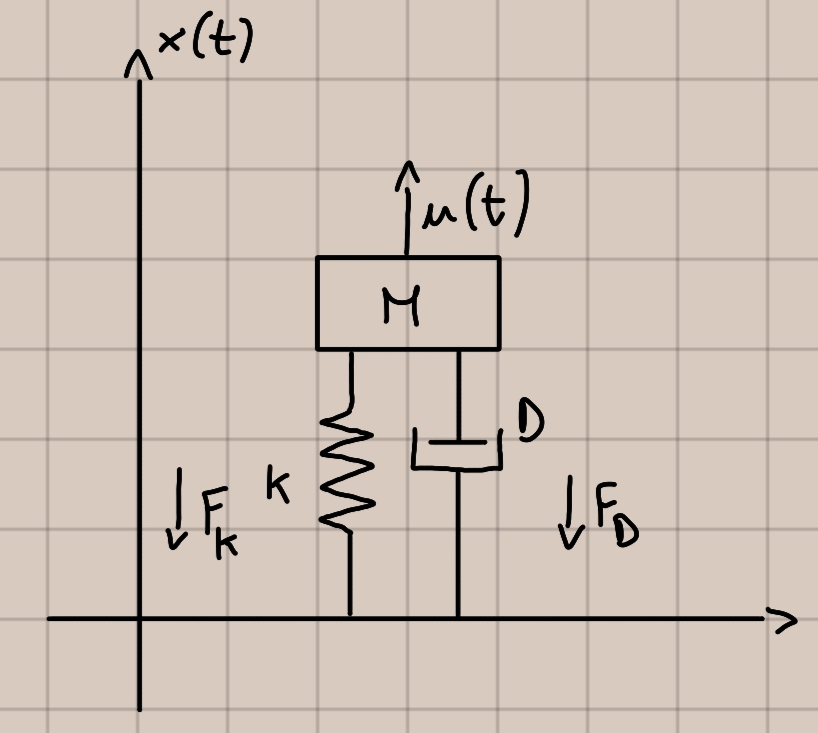
\includegraphics[width=0.5\textwidth]{molla.jpg}
\end{center}

Essendo che $F = ma$ e che $a(t) = \frac{d^2x(t)}{dt^2}$ avremo che:
\[
    \begin{split}
        &Ma(t) = u(t) - \underbrace{F_K}_{kx(t)} - \overbrace{F_D}^{D\frac{dx(t)}{dt}} \Rightarrow \\
        &\overbrace{M \frac{d^2x(t)}{dt^2} + D \frac{dx(t)}{dt} + kx(t)}^{ingresso} = \underbrace{u(t)}_{uscita} \\
    \end{split}
\]

Esempio 2: Circuito elettrico

\begin{center}
    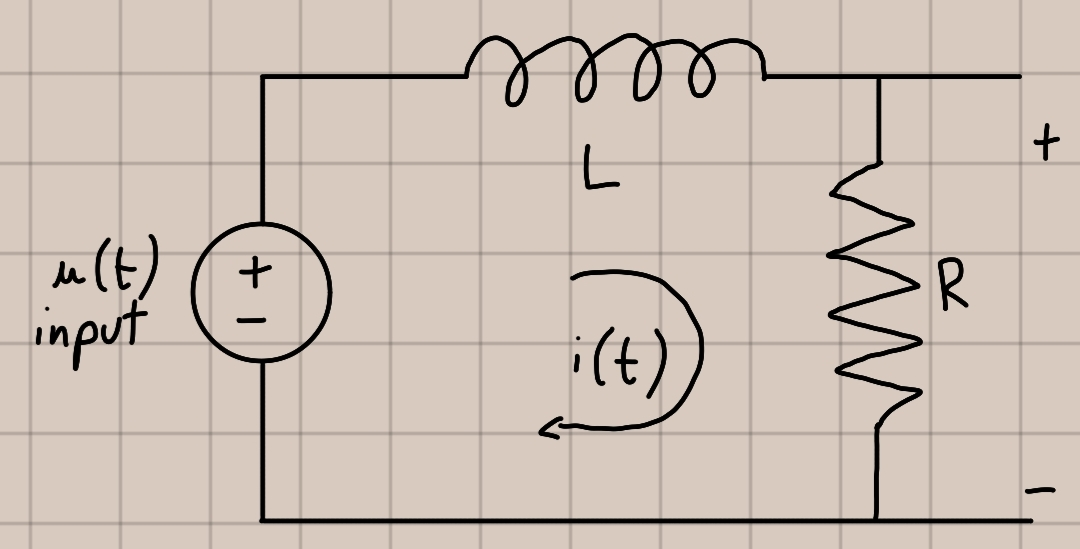
\includegraphics[width=0.5\textwidth]{circuito.jpg}
\end{center}

L'ingresso in questo caso è dato dalla tensione formata dalla somma delle tensioni sull'induttore e la resistenza, come output
avremo la tensione ai capi dei resistori:
\[
    \begin{split}
        &u(t) = L \frac{di(t)}{dt} + \underbrace{Ri(t)}_{v(t)} \\
        &\textrm{se } v(t) = Ri(t) \Rightarrow i(t) = \frac{1}{R} v(t) \\
        &\frac{L}{R} \frac{dv(t)}{dt} + v(t) = u(t) \\
    \end{split}
\]

In generale sono una sommatoria delle derivate dell'input che saranno uguali alla sommatoria delle derivate 
dell'output, in generale ha la seguente forma:

\[
    a_n \frac{d^nv(t)}{dt^n} + a_{n - 1} \frac{d^{n - 1}v(t)}{dt^{n - 1}} + \dots + a_1 \frac{dv(t)}{dt} + a_0 v(t) = b_m \frac{d^mu(t)}{dt^m} + b_{m - 1} \frac{d^{m - 1} u(t)}{dt^{m - 1}} + \dots + b_0u(t)
\]

dove $u(t)$ è l'ingresso, $v(t)$ è l'uscita e $a_n, b_n \neq 0$ è fondamentale che la derivata di ordine maggiore abbia 
coefficiente non nullo. L'equazione può essere riscritta in forma compatta con la sommatoria:

\[
    \sum_{i = 0}^n a_i \frac{d^iv(t)}{dt^i} = \sum_{i = 0}^m b_i \frac{d^iu(t)}{dt}
\]

$n$ si chiama l'ordine dell'equazione differenziale, in generale $n \ge m$, su tutti i sistemi considerati il grado 
di derivazione dell'output sarà maggiore o uguale dell'input. Se $n \ge m$ il sistema è detto \textbf{strettamente proprio}, altrimenti
il sistema è \textbf{proprio}.

Riprendendo gli esempi fatti sopra:

\[
    \underbrace{Mx''(t)}_{a_2} + \underbrace{Dx'(t)}_{a_1} + \underbrace{kx(t)}_{a_0} = \underbrace{u(t)}_{b_0}
\]

Possiamo notare che il sistema è strettamente proprio siccome $n = 2$ e $m = 0$

\begin{description}
    \item[Osservazione:] il sistema descritto con l'equazione differenziale non ha soluzione unica, a patto che non vengano imposte $n$ condizioni iniziali 
\end{description}

\subsection{Soluzione di un sistema a tempo continuo descritto da un'equazione differenziale}

La soluzione equivale all'uscita $v$ (reale o complessa) che si può scomporre in 

\[
    v = \underbrace{v_l}_{\textrm{risposta libera}} + \underbrace{v_f}_{\textrm{risposta forzata}}
\]

La risposta libera è la parte che non dipende dall'ingresso, ma dalle condizioni iniziali, perché il sistema può anche non essere a riposo, 
mentre la risposta forzata dipende dall'ingresso $u$. 

\paragraph{Evoluzione libera (oppure risposta libera)}

Per calcolare l'evoluzione libera associamo all'equazione differenziale iniziale l'equazione differenziale \textbf{omogenea}:

\[
    \sum_{i = 0}^n a_i \frac{d^iv(t)}{dt^i} = 0
\]

quando una parte dell'equazione viene posta a 0 l'equazione si definisce \textbf{omogenea}, all'equazione qui sopra 
associamo il \textbf{polinomio caratteristico}

\[
    P(s) = \sum_{i = 0}^n a_i s^i
\]

Devo risolvere l'equazione caratteristica $P(s) = 0$ applicando il teorema fondamentale dell'algebra $\rightarrow \lambda_1, \dots, \lambda_r$
sono radici di $P(s) = 0$ con le molteplicità $\mu_1, \dots, \mu_r$  con $\mu_1 + \dots + \mu_r = n$. La soluzione dell'equazione 
per il calcolo della risposta libera è:

\[
    v(t) = \sum_{i = 1}^r \sum_{l = 0}^{\mu_{i -1}} c_{i | l} e^{\lambda it} \frac{t^l}{l!}
\]

I coefficienti $c_{i | l}$ vengono determinati dalle condizioni iniziali. 

Esempio 1:

\[
    \begin{split}
        &Mx'' + Dx' + kx = 0 \quad M = 1 \quad D = 2 \quad k = 1 \\
        &P(s) = s^2 + 2s + 1 \quad \underbrace{\lambda_1 = -1}_{\textrm{valore che lo annulla}} \quad \underbrace{\mu_1 = 2}_{\textrm{ il grado}} \\
        &x(t) = \sum_{i = 1}^1 \sum_{l = 0}^1 c_{i , l} e^{-t} \frac{t^l}{l!} = \\
        &\sum_{l = 0}^1 c_{i , l} e^{-t} \frac{t^l}{l!} = \\
        &c_{1, 0} e^{-t} + c_{1, 1} e^{-t} t
    \end{split}
\]

Notare che la prima sommatoria non c'è perché abbiamo una sola radice distinta.

Esempio 2:

\[
    \begin{split}
        &v'''(t) + 3v''(t) + 3v'(t) + 1 = 0 \\
        &P(s) = s^3 + 3s^2 + 3s + 1 = (s + 1)^3 \\
        &\lambda_1 = 1 \quad \mu_1 = 3 \\
        &v(t) = c_{1,0} e^{-t} + c_{1,1} e^{-t}t + c{_1,2} e^{-t} \frac{t^2}{2}
    \end{split}
\]

La prima sommatoria scompare pure in questo caso.

\subsection{Modi elementari}

\[
    m_i(t) = e^{\lambda it} \frac{t^l}{l!}
\]

è detto \textbf{modo elementare} $(i = 1,\dots,r)$

\begin{description}
    \item[Osservazione:] $c_{i,l}$ verranno calcolati dalle condizioni iniziali. 
\end{description}

Esempio: Trovare la risposta libera del sistema

\[
    v''(t) + 3v'(t) - 4v(t) = 5u'(t) - u(t)
\]

con le condizioni iniziali

\[
    v(0) = 0, \quad v'(0) = 1
\]

Come si risolve? Si scrive l'equazione omogenea:

\[
    v''(t) + 3v'(t) - 4v(t) = 0
\]

Ora si scrive il polinomio caratteristico:

\[
    \begin{split}
        &P(s) = s^2 + 3s - 4 = (s - 1)(s + 4) \\
        &\lambda_1 = 1 \quad \mu_1 = 1 \\
        &\lambda_2 = -4 \quad \mu_2 = 1 \\
        &v_l(t) = c_{1,0} e^t + c_{2,0} e^{-4t} \\
        &v_l'(t) = c_{1,0} e^t - 4c{2,0}^{-4t} \\
    \end{split}
\]
\[
v_l(0) =
    \begin{cases}
        c_{1,0} + c_{2,0} = 0 \textrm{ condizione iniziale} \\
        c_{1,0} - 4c_{2,0} = 1 \textrm{ condizione iniziale} \\
    \end{cases}
\]
\[
    \begin{split}
        &c_{1,0} = \frac{1}{5} \quad c_{2,0} = -\frac{1}{5} \\
        &v_l(t) = \frac{1}{5} e^t - \frac{1}{5} e^{-4t}
    \end{split}
\]

Per un sistema descritto dall'equazione differenziale di base, la risposta libera è la funzione $v_l$ che si ottiene come 
soluzione dell'equazione omogenea 

\[
    \sum_{i = 1}^n a_i \frac{d^iv(t)}{dt^i} = 0
\]

i cui coefficienti sono determinati dalle condizioni iniziali.

\begin{description}
    \item[Osservazione:] la risposta libera di un sistema è la risposta del sistema in assenza di ingresso ($u(t) = 0$) e dipende soltanto dalla condizioni iniziali.
\end{description}

\subsection{Convergenza dei modi elementari}

Dato il modo elementare vale che:

\begin{enumerate}
    \item \[\lim_{t \rightarrow \infty} m(t) = 0 \Leftrightarrow Re(\lambda) < 0\]
    \item \[m(t) \textrm{ limitato su } [0, \infty) \Leftrightarrow Re(\lambda) \le 0\] Se $Re(\lambda) = 0$ allora deve valere che $l = 0$
    \item \[\lim_{t \rightarrow \infty} = \infty\] in tutti gli altri casi $(Re(\lambda) > 0)$ oppure $Re(\lambda) = 0$ e $l \neq 0)$
\end{enumerate}

\textbf{Dimostrazione:}

\begin{enumerate}
    \item $Re(\lambda) < 0$. Scriviamo \[\lambda = \sigma + j\omega \Rightarrow\] \[\begin{split}
        m(t) &= \frac{t^l}{l!}e^{\sigma t}e^{j\omega t} \\
        &\underbrace{\frac{t^l}{l!\overbrace{e^{-\sigma t}}^{\infty}}}_0 \overbrace{e^{j\omega t}}^{\textrm{funzione limitata}} \Rightarrow \\
        &\lim_{t \rightarrow \infty} m(t) = 0
    \end{split}\]
    \item $Re(\lambda) \le 0$ per $Re(\lambda) < 0$  abbiamo visto che il modo converge per \[t \rightarrow \infty \overbrace{\Rightarrow}^{m(t) \textrm{ continuo}} m(t) \textrm{ limitato }\] Per \[Re(\lambda) = 0 \textrm{ e } l = 0 \Rightarrow m(t) = e^{j\omega t}\] una funzione limitata in modulo;
    \item \[Re(\lambda) > 0 \Rightarrow e^{\sigma t} \rightarrow \infty \textrm{ per } t \rightarrow \infty \Rightarrow \lim_{t \rightarrow \infty} m(t) = \infty\] Per \[Re(\lambda) = 0 \textrm{ e } l \neq 0 \Rightarrow m(t) = \underbrace{\frac{t^l}{l!}}_{\textrm{per } t\rightarrow \infty = \infty} \underbrace{e^{j\omega t}}_{\textrm{limitata}} \Rightarrow \lim_{t \rightarrow \infty} m(t) = \infty\]
\end{enumerate}

\begin{description}
    \item[Teorema:] un sistema LTI descritto dall'equazione differenziale è asintoticamente stabile se e solo se ogni suo modo elementare converge a zero, cioè \[\lim_{t \rightarrow \infty} m_i(t) = 0, \textrm{ dove } m_i(t) = e^{\lambda it} \frac{t^l}{l!} \textrm{ per } i = 1, \dots, r\]
    \item[Osservazione:] un sistema LTI descritto  dall'equazione differenziale è asintoticamente stabile se e solo se tutte le radici del polinomi caratteristico hanno la parte reale negativa
\end{description}

\begin{SCfigure}[50][h!]
    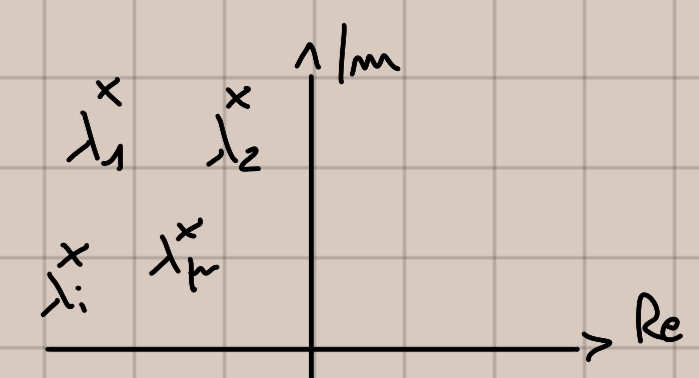
\includegraphics[width=0.5\textwidth]{radici.jpg}
    \caption{Con le radici a sinistra dell'asse dell'immaginario il sistema sarà asintoticamente stabile.}
\end{SCfigure}

\begin{SCfigure}[50][h!]
    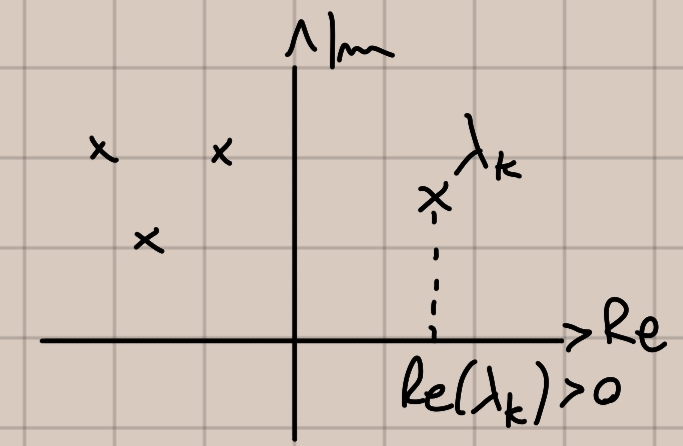
\includegraphics[width=0.5\textwidth]{radici2.jpg}
    \caption{Questo sistema non è asintoticamente stabile perché ho una parte reale maggiore di zero.}
\end{SCfigure}

Esempio 1 dal circuito eletrico RL:

\[
    \frac{dv(t)}{d(t)} + \frac{R}{L}v(t) = \frac{R}{L}u(t)
\]

L'equazione caratteristica sarà:

\[
    s + \frac{R}{L} = 0 \Rightarrow \lambda = -\frac{R}{L} \in R \quad \lambda < 0 \textrm{ per } R,L>0
\]

quindi il sistema è stabile.

Esempio 2 della molla:

\[
    M\frac{d^2v(t)}{dt^2} + D\frac{dv(t)}{dt} - kv(t) = 0 \textrm{ con } M, D, k > 0
\]

L'equazione caratteristica sarà:

\[
    Ms^2 + Ds - k = 0 \rightarrow \lambda_{1,2} = \frac{-D\pm \sqrt{D^2 + 4kM}}{2M}
\]

In base ai valori di M, D, k si ricaveranno i valori di $\lambda_1, \lambda_2$

\subsection{Risposta impulsiva ed evoluzione forzata}

\begin{description}
    \item[Definizione:] il prodotto di convoluzione tra due funzione u,v se esiste è definito da \[\begin{split}
        (u \ast v)(t) &= \int_{-\infty}^\infty u(\xi)v(t - \xi)d\xi = \\
        &\underbrace{=}_{\textrm{cambio variabile } t - \xi = x} \int_{-\infty}^\infty u(t - \xi)v(\xi)d\xi 
    \end{split}\] 
\end{description}

Proprietà:
\begin{enumerate}
    \item Commutatività: \[(u \ast v)(t) = (v \ast u)(t)\]
    \item Associatività: \[(u \ast v)(t) \ast w(t) = u(t) \ast (v \ast w)(t)\]
    \item Distribuibilità rispetto alla somma: \[u(t) \ast (v(t) + w(t)) = (u \ast v)(t) + (u \ast w)(t)\] questre tre prime proprietà derivano dalle proprietà dell'integrazione
    \item L'impulso è elemento neutro per la convoluzione: \[(v \ast \delta)(t) = (\delta \ast v)(t) = v(t)\] per la proprietà di campionamento dell'impulso: \[v(t) = \int_{-\infty}^\infty v(\xi)\delta(t - \xi)d\xi = (v \ast \delta)(t)\] 
\end{enumerate}

\begin{description}
    \item[Definizione:] dato un sistema a tempo continuo inizialmente a riposo definiamo la risposta impulsiva del sistema, la risposta in corrispondenza dell'impulso ideale 
\end{description}

\begin{SCfigure}[50][h!]
    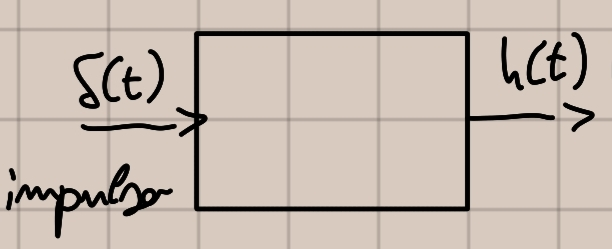
\includegraphics[width=0.5\textwidth]{risposta_impulsiva.jpg}
    \caption{La risposta impulsiva $h(t)$}
\end{SCfigure}

\begin{description}
    \item[Teorema:] la risposta in uscita $v(t)$ di una sistema LTI, inizialmente a riposo , in corrispondenza a un ingresso $u(t)$ è data dal seguente prodotto di convoluzione (se esiste) \[v(t) = (u \ast h)(t) = \int_{-\infty}^\infty h(\xi)u(t - \xi)d\xi = \int_{-\infty}^\infty h(t - \xi) u(\xi) d\xi\] con $h(t)$ la risposta impulsiva del sistema.
    \item[Osservazione:] un sistema LTI inizialmente a riposo è causale \[u(t) = 0, v(t) = 0 \textrm{ per } t < 0\] siamo a riposo. Siccome $h(t) = 0$ per $t < 0$ (perché $\delta (t) = 0, t < 0) \Rightarrow$ \[\begin{split}
        (u \ast h)(t) &= \int_{0^-}^\infty h(\xi) u(t - \xi) d\xi = \\
        &= \int_{-\infty}^{t^+} h(t- \xi) u(\xi) d\xi
    \end{split} \] In particolare, la risposta forzata di un sistema LTI, iniziailmente a riposo (quindi causale) in corrispondenza a un ingresso $u(t) (u(t) = 0, t<0)$ è: \[ \begin{split}
        v_f(t) = (u \ast h) (t) &= \int_{0^-}^{t^+} h(\xi) u(t - \xi) d\xi = \\
        &= \int_{0^-}^{t^+} h(t - \xi) u(\xi) d\xi
    \end{split}\]
    \item[Dimostrazione:] \begin{SCfigure}[50][h!]
        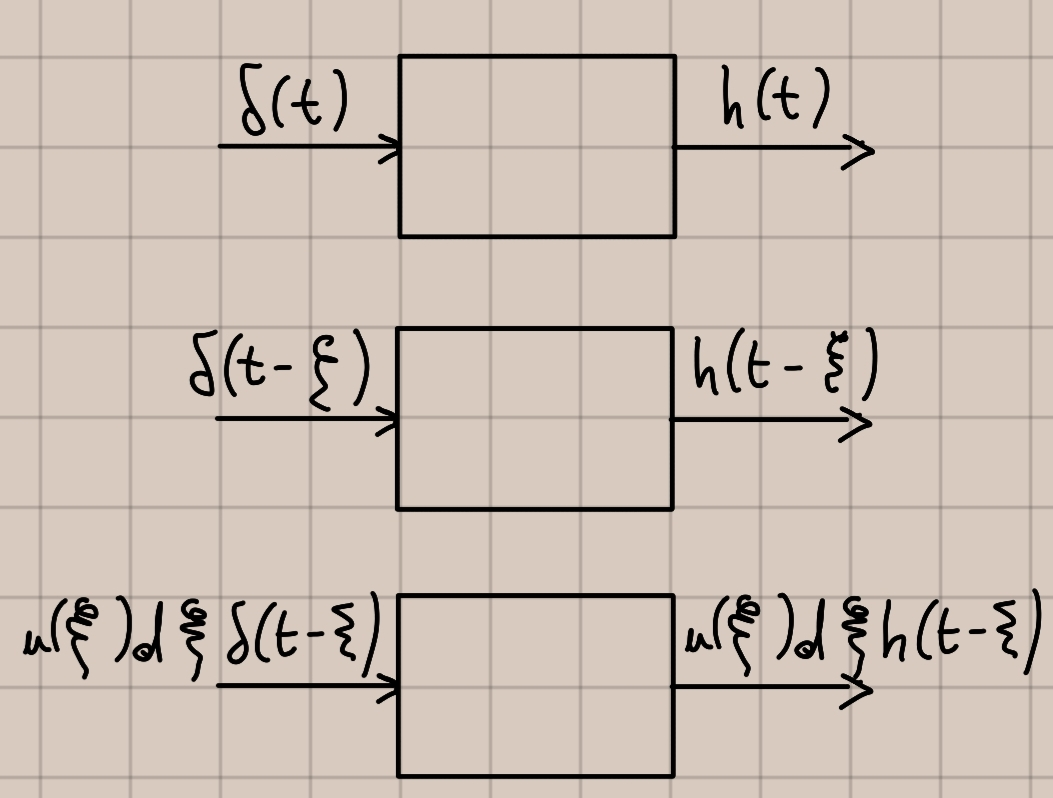
\includegraphics[width=0.5\textwidth]{tre_sistemi.jpg}
        \caption{La secondo valida per tempo invarianza, mentre la terza per la linearità }
    \end{SCfigure} Integriamo $\Rightarrow$ \[ \begin{split}
        &\underbrace{\int_{-\infty}^\infty u(\xi) \delta(t - \xi) d\xi}_{u(t)} \mapsto \int_{-\infty}^\infty u(\xi) h(t - \xi) d\xi \\
        &u(t) \mapsto \int_{-\infty}^\infty u(\xi) h(t - \xi) d\xi = (u \ast h)(t)
    \end{split} \]
    \begin{SCfigure}[50][h!]
        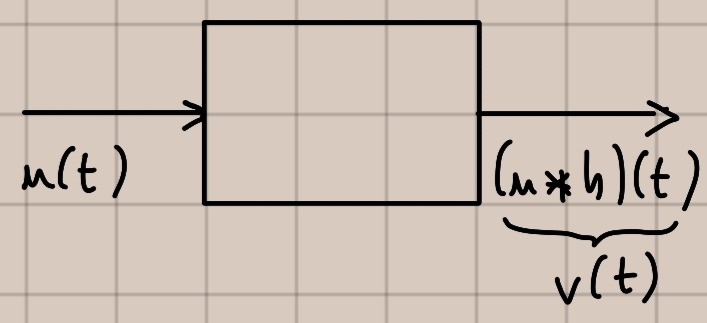
\includegraphics[width=0.5\textwidth]{sistema1.jpg}
        \caption{Dimostrazione completata.}
    \end{SCfigure}
    \item[Osservazione:] si può dimostrare che per il sistema definito dalla prima equazione differenziale \[h(t) = d_0\delta(t) + \sum_{i = 1}^r \sum_{l = 0}^{\mu_i - 1} d_{i,l} \frac{t^l}{l!} e^{\lambda_it} \underbrace{\delta_{-1} (t)}_{\textrm{dobbiamo assicurarci la causalità}}\] con $d_0 \neq 0$ se e solo se $n = m$ 
\end{description}

Esempio: determinare la risposta impulsiva del sistema 

\[
    \frac{dv(t)}{dt} + 2v(t) = \frac{du(t)}{dt} + u(t)
\]

Equazione caratteristica:

\[
    s + 2 = 0 \Rightarrow \lambda = -2 \Rightarrow \textrm{ il modo elementare } m(t) = e^{-2t}
\]

\[
    h(t) = d_0\delta(t) + d_1 e^{-2t} \delta_{-1} (t)
\]

Come si ricavano $d_0, d_1= ?$

\[
    \frac{dh(t)}{dt} = d_0 \frac{d\delta(t)}{dt} -2d_1 e^{-2t} \delta_{-1}(t) + d_1 e^{-2t} \delta(t)
\]

Sostituisco nell'equazione (*)

\[
    \begin{split}
        \Rightarrow &d_0 \frac{d\delta(t)}{dt} - 2d_1 e^{-2t} \delta_{-1}(t) + d_1 e^{-2t} \delta(t) + 2d_0 \delta(t) + 2 d_1 e^{-2t} \delta_{-1}(t) = \frac{d\delta(t)}{dt} +\delta(t) \\
        &d_0 \frac{d\delta(t)}{dt} + d_1 \delta(t) + 2d_0 \delta(t) = \frac{d\delta(t)}{dt} + \delta(t) \\
        &d_{0 - 1} \frac{d\delta(t)}{dt} + (d_1 + 2d_{0 - 1}) \delta(t) = 0 \\
    \end{split}
\]
\[\Rightarrow
\begin{cases}
    d_{0 - 1} = 0 \Rightarrow d_0 = 1\\
    d_1 + 2d_{0 - 1} = 0 \Rightarrow d_1 = -1\\
\end{cases}
\]
Per $t\rightarrow 0$. Perciò abbiamo trovato la nostra risposta impulsiva:

\[
    h(t) = \delta(t) - e^{-2t} \delta_{-1}(t)
\]

Riassumento, se noi abbiamo una sistema LTI rappresentato dall'equazione differenziale, avremo che la risposta totale sarà data dalla somma della risposta libera con la risposta forzata:

\[
    v(t) = v_l(t) + v_f(t)
\]

\begin{itemize}
    \item $v_l(t)$ si ottiene trovando le radici dell'equazione omogenea associata e utilizzando le condizioni iniziali $\rightarrow$ stabilità asintotica
    \item $v_f(t)$ si ottiene tramite \[\int_0^{t^+} u(\xi)h(t - \xi) d\xi\] $\rightarrow$ stabilità BIBO
\end{itemize}

\subsection{Stabilità di un sistema continuo definito dalla risposta impulsiva}

\begin{description}
    \item[Teorema:] un sistema a tempo continuo LTI è BIBO stabile se e solo se \[ \int_{-\infty}^\infty |h(\xi)|d\xi < \infty\]
    \item[Dimostrazione:] da destra a sinistra, se \[\int_{-\infty}^\infty |h(\xi)|d\xi < \infty \Rightarrow \textrm{ il sistema è BIBO stabile}\] Se l'ingresso $u(t)$ tale che $|u(t)| < M_u, \forall t$ dobbiamo dimostrare che l'uscita $v(t)$ corrispondente  è limitata $(\exists M_v \textrm{ t.c. } |v(t)| < M_v, \forall t)$ \[ \begin{split}
        &v(t) = (u \ast h)(t) = \int_{-\infty}^\infty h(\xi) u(t - \xi) d\xi \\
        &|v(t)| = \int_{-\infty}^\infty |h(\xi) u(t - \xi)| d\xi = \\
        &= \int_{-\infty}^{\infty} |h(\xi)|\underbrace{|u(t - \xi)|}_{< M_u} d\xi < \overbrace{M_u \underbrace{\int_{-\infty}^\infty|h(\xi)|d\xi}_{< \infty}}^{= M_v} \\
        &\Rightarrow |v(t)| < M_v
    \end{split} 
    \]
\end{description}

\subsection{Risposta in frequenza}

Ci interessa la risposta di un sistema definito dall'equzione differenziale
in corrispondenza di un ingresso del tipo: 

\[
    u(t) = A e^{j(\omega_0t + \phi)} = A e^{j\phi} e^{j\omega_0t} \quad (fasore)
\]
Il sistema è BIBO stabile $\leftrightarrow$ 
\[
    \int_{-\infty}^\infty |h(\tau)| d\tau < +\infty
\]
\[
\begin{split}
    v(t) &= (u \ast h)(t) = \int_{-\infty}^\infty h(\tau) u(t - \tau) d\tau = \\
    &= \int_{-\infty}^\infty h(\tau) A e^{j(\omega_0(t - \tau) +)} d\tau = \\
    &= \underbrace{A e^{j(\omega_0t + \phi)}}_{\in C} \underbrace{\int_{-\infty}^\infty h(\tau) e^{-j\omega_0\tau)} d\tau}_{\textrm{converge?}} \\
    &|\int_{-\infty}^\infty h(\tau) e^{-j\omega_0\tau} d\tau| = \int_{-\infty}^\infty |h(\tau)| |\underbrace{e^{-j \omega_0 \tau}}_{= 1}| d\tau = \\
    &= \int_{-\infty}^\infty |h(\tau)| d\tau < +\infty
\end{split}
\]
Possiamo scrivere:
\[
    \begin{split}
        &H(j\omega_0) = \int_{-\infty}^\infty h(\tau) e^{-j\omega_0 \tau} d\tau \\
        &\Rightarrow v(t) = \underbrace{H(j\omega_0)}_{\textrm{dipende soltanto dal sistema considerato}} \underbrace{A e^{j(\omega_0 t + \phi)}}_{\textrm{l'ingresso}}, t \in R
    \end{split}
\]
\begin{description}
    \item[Definizione:] dato un sistema LTI BIBO stabile, di risposta impulsiva h(t) definiamo la \textbf{rispsta in frequenza} la 
    funzione \[ H(j\omega) =   \int_{-\infty}^\infty h(\tau) e^{-j\omega \tau} d\tau, H(j\omega) \in C, \omega \in R \] Definiamo inoltre
    \[ \begin{split}
        &A(\omega) = |H(j\omega)| \\
        &\Phi(\omega) = arg(H(j\omega))
    \end{split}
    \] il modulo A e l'argomento (la fase) $\Phi$ della rispota in frequenza H 
    \[\begin{split}
        &A(\omega) := |H(j\omega)| = |\int_{-\infty}^\infty h(\tau) e^{-j\omega \tau)} d\tau| \\
        &\Phi(\omega) := arg(H(j\omega)) = arg(\int_{-\infty}^\infty h(\tau) e^{-j\omega \tau} d\tau)
    \end{split}
    \]
\end{description}
\begin{figure}[h!]
    \centering
    \subfloat[][]
    {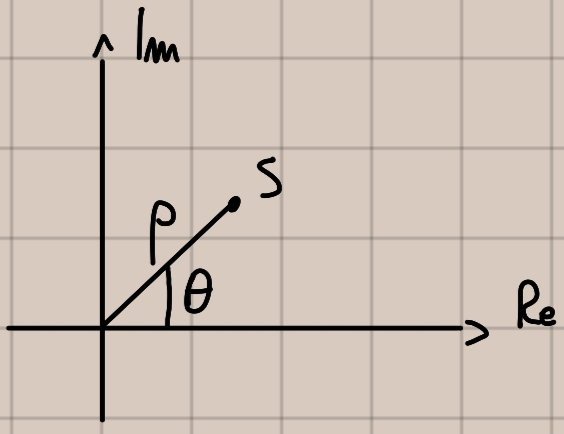
\includegraphics[width=0.5\textwidth]{risp_freq1.jpg}}\quad
    \subfloat[][]
    {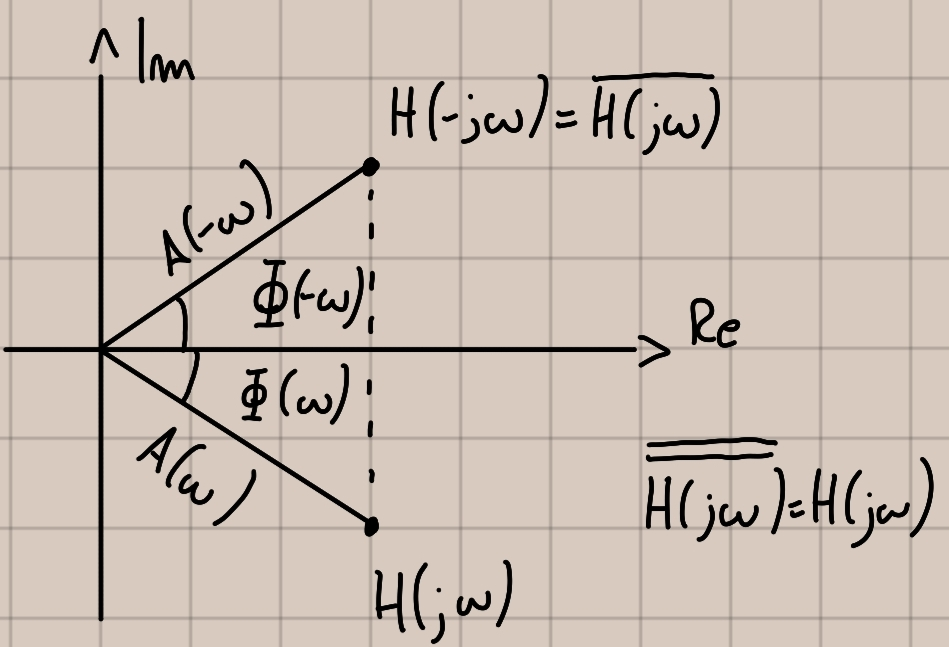
\includegraphics[width=0.5\textwidth]{risp_freq2.jpg}}
\end{figure}
\[
    \begin{split}
        &s = \rho(\cos \theta + j \sin \theta) \\
        &\rho = |s| \\
        &\theta = arg(s)
    \end{split}
\]
Proprietà:
\begin{enumerate}
    \item $A(\omega)$ è pari $(A(-\omega) = A(\omega))$
    \item $\Phi(\omega)$ è dispari $(\Phi(-\omega) = -\Phi(\omega))$
    \item $H(-j\omega)$ = $\overline{H(j\omega)}$ 
\end{enumerate}
\textbf{Dimostrazione del punto 3}
\[
    \begin{split}
        H(-j \omega) &= \int_{-\infty}^\infty \underbrace{h(\tau)}_{\in R} e^{j \omega \tau} d \tau = \\
        &= \int_{-\infty}^\infty \overline{h(\tau) e^{-j \omega \tau}} d \tau = \\
        &= \overline{\int_{-\infty}^\infty h(\tau) e^{-j \omega \tau} d \tau} = \overline{H(j \omega)}
    \end{split}
\]
Esempio di risposta a un segnale sinusoidale:
\[
    u(t) = A \cos (\omega t + \underbrace{\phi}_{fase})
\]
Formula di Eulero
\[
    \begin{split}
        \Rightarrow u(t) &= \frac{A}{2} e^{j(\omega t + \phi)} + \frac{A}{2} e^{-j(\omega t + \phi)} = \\
        &= \underbrace{\frac{A}{2} e^{j \phi} e^{j \omega t}}_{u_1(t)} + \underbrace{\frac{A}{2} e^{-j \phi} e^{-j \omega t}}_{u_2(t)}
    \end{split}
\]
Per la linearità 
\[
    \begin{split}
        &u_1(t) \mapsto v_1(t) \\
        &u_2(t) \mapsto v_2(t) 
    \end{split}
\]
Quindi 
\[
    A \cos (\omega t + \phi) = u_1(t) + u_2(t) \mapsto v_1(t) + v_2(t) = v(t)
\]
Scriviamo
\[
    \begin{split}
        &H(j \omega) = A(\omega) e^{j \phi (\omega)} \textrm{ rappresentazione esponenziale} \\
        v(t) &= \underbrace{\frac{A}{2} A(\omega) e^{j(\phi + \Phi (\omega))} e^{j \omega t}}_{v_1(t)} + \underbrace{\frac{A}{2} A(-\omega) e^{-j(\phi - \Phi (-\omega))} e^{-j \omega t}}_{v_2(t)} = \textrm{ per proprietà 1 e 2} \\
        &= A(\omega) \frac{A}{2} e^{j(\phi + \Phi (\omega))} e^{j \omega t} + \frac{A}{2} A(\omega) e^{-j(\phi + \Phi (\omega))} e^{-j \omega t} \\
        &= AA(\omega)[\frac{e^{j(\omega t + \phi + \Phi(\omega))}}{2} + \frac{e^{-j(\omega t + \phi + \Phi(\omega))}}{2}] = \\
        &= AA(\omega) \cos (\omega t + \phi + \Phi (\omega)) \\
        &\underbrace{A \cos (\omega t + \phi)}_{ingresso} \mapsto \underbrace{\overbrace{AA(\omega)}^1 \cos (\omega t + \phi + \overbrace{\Phi (\omega)}^2)}_{uscita}
    \end{split}
\]
\begin{enumerate}
    \item Per l'ampiezza della risposta in frequenza $H(j \omega)$
    \item Più l'argomento (fase) della risposta in frequenza $H(j \omega)$
\end{enumerate}
\begin{description}
    \item[Osservazione:] La risposta di un sistema LTI e BIBO staile a un segnale sinusoidale di frequenza $\omega$ e un 
    segnale sinusoidale della stessa frequenza $\omega$ è:
    \begin{itemize}
        \item ampiezza data dal prodotto dell'ampiezza dell'ingresso per l'ampiezza della risposta in frequenza;
        \item fase data dalla somma della fase iniziale e della fase della risposta in frequenza
    \end{itemize}   
\end{description}

Esempio $u(t) = e^{j \omega t}$
\[
    \begin{split}
        v(t) = (u \ast h) (t) &= \int_{-\infty}^\infty h(\tau)  e^{j \omega (t - \tau)} d \tau = \\
        &= e^{j \omega t} \underbrace{\int_{-\infty}^\infty h(\tau)  e^{-j \omega \tau} d \tau}_{H(j \omega) \textrm{ risposta in frequenza}} = H(j \omega) e^{j \omega t}
    \end{split}
\]
Per i sistemi definiti dall'equazione differenziale e ingresso $u(t)$
\[
    \begin{split}
        &\sum_{i = 0}^n a_i \frac{d^iv(t)}{dt^i} = \sum_{i = 0}^m b_i \frac{d^iu(t)}{dt^i} \\
        &\Rightarrow \sum_{i = 0}^n a_i \frac{d^i (H(j \omega) e^{j \omega t})}{dt^i} = \sum_{i = 0}^m b_i \frac{d^i (e^{j \omega t})}{dt^i} \\
        &\Leftrightarrow H(j \omega) e^{j \omega t} \sum_{i = 0}^n a_i (j \omega)^i =  e^{j \omega t} \sum_{i = 0}^m b_i (j \omega)^i \\
        &\frac{d^i (e^{j \omega t})}{dt^i} = (j \omega)^i e^{j \omega t}
    \end{split}
\]
\begin{description}
    \item[Osservazione:] Per il sistema dell'equazione differenziale, in corrispondenza di ingressi fasori la risposta in 
    frequenza è una funzione razionale (rapporto di due polinomi) in $j\omega$. 
\end{description}

\subsection{La trasformata di Laplace}

Sia $v(t), t \in R$ una funzione sommabile su $[0^-, \infty)(\int_{-\infty}^\infty |v(t)| dt < \infty)$ la \textbf{trasformata 
di Laplace unilatera} è:
\[
    V(s) = \int_{-\infty}^\infty v(t) e^{-st} dt, s \in C
\]
Notazione $V(s) = \mathcal{L} [v(t)](s)$
\begin{description}
    \item[Osservazione:] Affinchè $V(s)$ esista \[ |\int_{0^-}^\infty v(t) e^{-st}| < \infty \textrm{ l'integrale converge} \] 
    Il dominio di $V$ saranno tutti gli $s$ per cui l'integrale converge e viene chiamato \textbf{regione di convergenza}(RdC).
    Si può dimostrare che RdC è sempre un semipiano aperto del tipo \[ RdC = {s \in C | Re(s) > \alpha}, \alpha \in R \] $\alpha$ 
    si chiama \textbf{ascissa di convergenza}.  
\end{description}
\begin{center}
    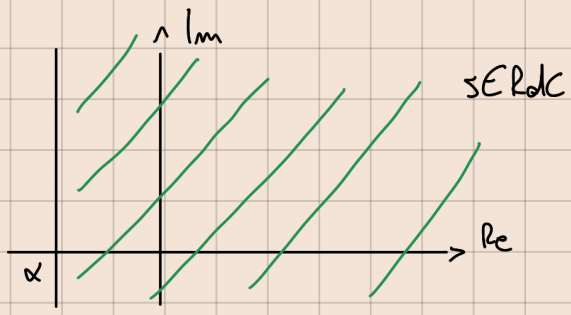
\includegraphics[width=0.5\textwidth]{RdC.png}
\end{center}

\subsection{RdC della trasformata di Laplace unilatera di una combinazione lineare di funzioni esponenziali}

\textbf{Teorema} $v(t) = \sum_{i = 0}^n c_i e^{\lambda_i t}$, dove $\lambda_i = \sigma_i + j \omega_i \in C$, $c_i$ costanti.
La RdC di $\mathcal{L} [v(t)] (s)$ è un semipiano destro 
\[
    RdC = { s \in C | Re(s) > \alpha} \textrm{ dove } \alpha = max{Re(\lambda_0), \dots, Re(\lambda_n)}
\]
Dimostrazione:
\[
    \begin{split}
        \mathcal{L} [v(t)] (s) &= \int_{0^-}^\infty (\sum_{i = 0}^n c_i e^{\lambda_i t}) e^{-st} dt = \\
        &\sum_{i = 0}^n c_i \int_{0^-}^\infty e^{\lambda_i t} e^{-st} dt \\
        &\int_{0^-}^\infty e^{}
    \end{split}
\]
\textbf{INCOMPLETA VEDI LEZIONE 31-03}
Per $i \in {o, \dots, n}$ sia $\lambda_i = \sigma_i + j\omega_i$ e $s = \sigma + j\omega$, valutiamo il modulo dell'integrale 
\[
    \begin{split}
        &| \int_{0^-}^\infty e^{\lambda_i t} e^{-st} dt | = \\
        &| \int_{0^-}^\infty e^{\sigma_i t} e^{j \omega_i t} e^{-\sigma t} e^{-j\omega t} dt | = \\
        &| \int_{0^-}^\infty e^{[\sigma_i - \sigma + j(\omega_i - \omega)]t} dt | = \\
        &| \frac{e^{[\sigma_i - \sigma + j(\omega_i - \omega)]t}}{\sigma_i - \sigma + j\omega_i - j\omega} |_{0^-}^\infty | = \\
        &| \lim_{t \rightarrow \infty} \frac{\overbrace{e^{(\sigma_i - \sigma)t}}^1 \overbrace{e^{j(\omega_i - \omega)t}}^2}{\sigma_i - \sigma + j\omega_i - j\omega} - \frac{1}{\sigma_i - \sigma + j\omega_i - j\omega} | < \infty \\
        & \textrm{per } \sigma > sigma_i \leftrightarrow Re(s) > Re(\lambda_i)
    \end{split}
\]
\begin{enumerate}
    \item converge per $\sigma_i - \sigma < 0$
    \item ha il modulo 1
\end{enumerate}
\begin{center}
    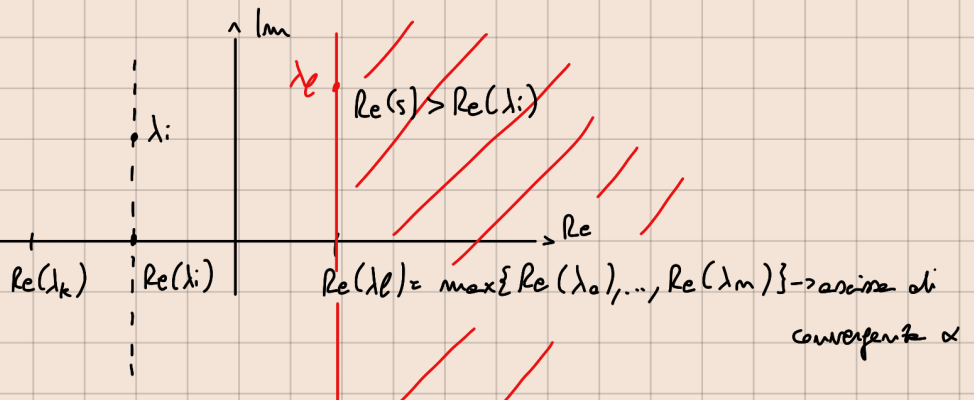
\includegraphics[width=0.5\textwidth]{RdC2.png}
\end{center}

\subsection{Proprietà della trasformata di Laplace}

\begin{enumerate}
    \item \textbf{Linearità}, se $v_1, v_2$ ammettono la trasformata di Laplace (TdL) allora anche $a_1v_1 + a_2v_2$ ammette la TdL e: \[ \mathcal{L} [a_1v_1(t) + a_2v_2(t)] (s) = a_1 \mathcal{L} [v_1(t)] (s) + a_2 \mathcal{L} [v_2(t)] (s) \] e l'ascissa di convergenza è $\alpha \ge max{\alpha_1, \alpha_2}$ dove $\alpha_1$ w $\alpha_2$ sono rispettivamente le ascisse di convergenza di $v_1$ e $v_2$ \begin{center}
        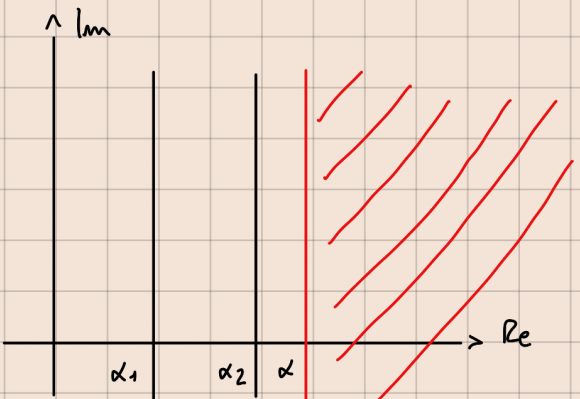
\includegraphics[width=0.5\textwidth]{RdC3.png}
    \end{center}
    \item Traslazione nel dominio del tempo (\textbf{time shifting}) se $v(t)$ ammette TdL allora anche $v(t - \tau), \tau > 0$ ammette TdL e:
    \[
        \mathcal{L} [v(t - \tau)] (s) = e^{-s \tau} \mathcal{L} [v(t)] (s)
    \]
    L'ascisse di convergenza non cambia
    \begin{center}
        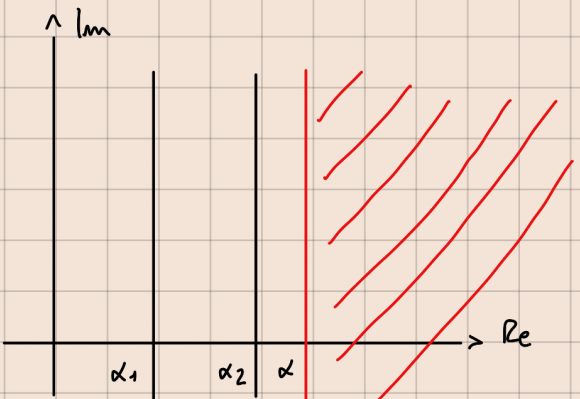
\includegraphics[width=0.5\textwidth]{RdC3.png}
    \end{center}
    \textbf{dimostrazione: } 
    \[
        \begin{split}
            \mathcal{L} [v(t - \tau)] (s) &= \int_{0^-}^\infty v(t - \tau) e^{-st} dt \overbrace{=}^* \\
            &= \int_{0^-}^\infty v(x) e^{-s(x + \tau)} dx = \\
            &= e^{s\tau} \int_{0^-}^\infty v(x) e^{-sx} dx \overbrace{=}^{**} \\
            &= e^{s \tau} \mathcal{L} [v(t)] (s)
        \end{split}
    \]
    (*) cambio di variabile \[x = t - \tau \Rightarrow dx = dt\]
    (**) ritorno alla variabile di prima
    \item Traslazione nel dominio dei complesi o moltiplicazione per una funzione esponenziale(\textbf{frequency shifting})
    Se $v(t)$ ammette TdL $V(s)$, allora anche $e^{\lambda t}v(t)$ ammette TdL e 
    \[
        \mathcal{L} [e^{\lambda t} v(t)] (s) = V(s - \lambda) (= \mathcal{L} [v(t)] (s- \lambda))
    \]
    L'ascissa di convergenza è $\alpha = \alpha_0 + Re(\lambda)$ dove $\alpha_0$ è l'ascissa di convergenza di $V(s)$ \textbf{dimostrazione:}
    \[
        \begin{split}
            \mathcal{L} [e^{\lambda t} v(t)] (s) &= \int_{0^-}^\infty e^{\lambda t} v(t) e^{-st} dt = \\
            &= \int_{0^-}^\infty v(t) e^{-(s - \lambda)t} dt = \mathcal{L} [v(t)] (s - \lambda) = V(s - \lambda)
        \end{split}
    \]
    \item Cambiamento di scale (\textbf{scaling}) se $v(t)$ ammette TdL allora $v(rt)$ ammette TdL e 
    \[
        \mathcal{L} [v(rt)] (s) = \frac{1}{r} V(\frac{s}{r})
    \]
    con ascissa di convergenza $\alpha = r \alpha_0$
    \begin{center}
        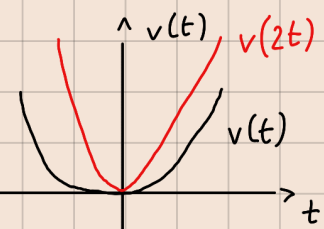
\includegraphics[width=0.5\textwidth]{RdC4.png}
    \end{center}
    \textbf{dimostrazione:}
    \[
        \begin{split}
            \mathcal{L} [v(rt)] (s) &= \int_{0^-}^\infty v(rt) e^{-st} dt \overbrace{=}^* \\
            & \frac{1}{r} \int_{0^-}^\infty v(\tau) e^{\frac{s}{r} \tau} d \tau = \\
            &\frac{1}{r} V(\frac{s}{r})
        \end{split}
    \]
    (*) cambio variabile \[ rt = \tau \quad dt = \frac{d\tau}{r}\]
\end{enumerate}




\end{document}